\documentclass[10pt,aspectratio=149]{beamer}

% All the boilerplate is in raslides.sty
% Note that this also pulls in a custom vogtwidebar.sty
\usepackage{raslides}

\author{Ji\v{r}\'i Lebl}

\institute[OSU]{%
Departemento pri Matematiko de Oklahoma {\^S}tata Universitato}

\title{BA: 2.3}

\date{}

\begin{document}

\begin{frame}
\titlepage
\end{frame}

\begin{frame}
\textbf{Example:}
$\bigl\{ {(-1)}^n \bigr\}_{n=1}^\infty$ is bounded but divergent.

\pause
But there are convergent subsequences converging to $-1$ and $1$.

\pause
Let's get at these limits.

\medskip
\pause

If $\{ x_n \}_{n=1}^\infty$ is bounded, then for every $n \in \N$, the set $\{ x_k : k \geq n \}$
is bounded.

\pause

\begin{definition}
Let $\{ x_n \}_{n=1}^\infty$ be a bounded sequence.

\medskip
\pause

Define
$a_n \coloneqq \sup \{ x_k : k \geq n \}$ and
$b_n \coloneqq \inf \{ x_k : k \geq n \}$.

\medskip
\pause

Define, if the limits exist,

\medskip

\quad
$\displaystyle
\limsup_{n \to \infty} x_n \coloneqq \lim_{n \to \infty} a_n$,
\qquad
$\displaystyle
\liminf_{n \to \infty} x_n \coloneqq \lim_{n \to \infty} b_n$.
\end{definition}

\pause

$\limsup$ is called \emph{limit superior} and
$\liminf$ is called \emph{limit inferior}.

\end{frame}

\begin{frame}

\textbf{Example:}
Consider $\{x_n\}_{n=1}^\infty$:

\medskip

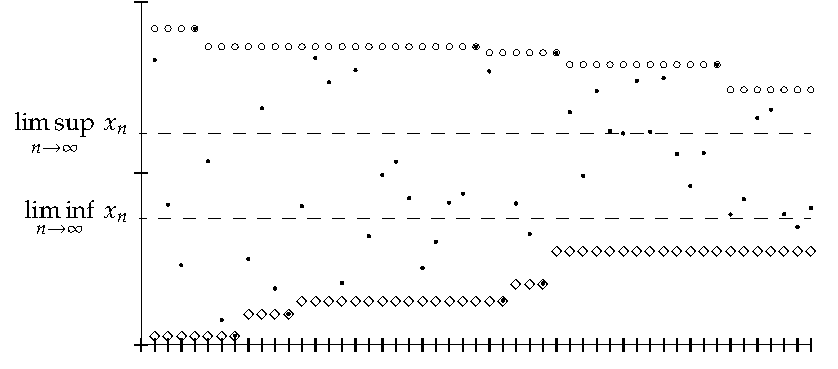
\includegraphics[width=4.5in]{../figures/sequence-limsupliminf_an_bn}

\medskip

$x_n$ are marked with dots (\raisebox{0.25ex}{\tiny$\bullet$}),

$a_n$ are marked with circles ($\circ$),

$b_n$ are marked with diamonds ($\diamond$).

\end{frame}

\begin{frame}

\begin{proposition}
Let $\{ x_n \}_{n=1}^\infty$ be a bounded sequence.  Let $a_n$ and $b_n$ be
as above.
\pause
\begin{enumerate}[(i)]
\item
$\{ a_n \}_{n=1}^\infty$ is bounded monotone decreasing
and $\{ b_n \}_{n=1}^\infty$ is bounded monotone increasing.  In particular,
$\liminf\limits_{n\to\infty} x_n$ and $\limsup\limits_{n\to\infty} x_n$ exist.
\item\pause
$\displaystyle \limsup_{n \to \infty} x_n = \inf \{ a_n : n \in \N \}$
and
$\displaystyle \liminf_{n \to \infty} x_n = \sup \{ b_n : n \in \N \}$.
\item\pause
$\displaystyle \liminf_{n \to \infty} x_n \leq
\limsup_{n \to \infty} x_n$.
\end{enumerate}
\end{proposition}

\pause

\textbf{Proof:}
(i) $a_n = \sup \{ x_k : k \geq n \}$ ~\thus~ $a_n$ is an upper bound for
$\{ x_k : k \geq (n+1) \}$

%\medskip
\pause

\thus \quad $a_{n+1} \leq a_n$ for all $n$.
%\medskip
\pause
\quad
Similarly for $\{ b_n \}_{n=1}^\infty$ (exercise).

\pause
\medskip

\textbf{Exercise:}
$\{a_n \}_{n=1}^\infty$ and $\{ b_n \}_{n=1}^\infty$ bounded.

\pause
\medskip

(ii) follows from (i).

\pause
\medskip

(iii)
$b_n \leq a_n$ for all $n$ \quad ($\inf \leq \sup$ for a nonempty set)

\pause
$b_n \to \liminf\limits_{n\to\infty} x_n$ \quad
and \quad $a_n \to \limsup\limits_{n\to\infty} x_n$
\pause
\wthus $\liminf\limits_{n\to\infty} x_n \leq \limsup\limits_{n\to\infty} x_n$ \qed

\end{frame}

\begin{frame}

\hspace*{2.3in}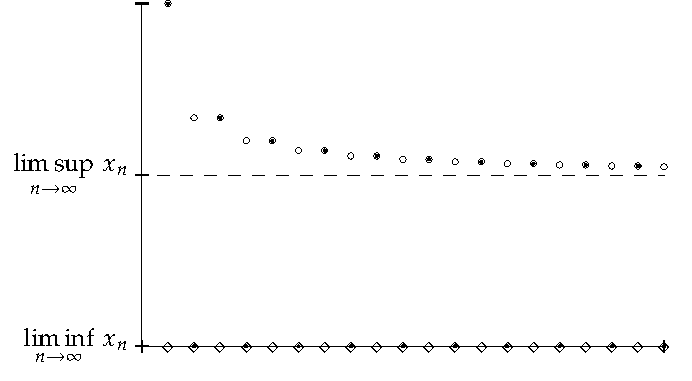
\includegraphics[width=2.6in]{../figures/sequence-limsupliminf_an_bn-example}

\vspace*{-1.5in}

\textbf{Example:}
Consider $\{ x_n \}_{n=1}^\infty$,

\medskip

$\displaystyle
x_n \coloneqq
\begin{cases}
\frac{n+1}{n} & \text{if } n \text{ is odd,} \\
0             & \text{if } n \text{ is even.}
\end{cases}
$

\pause
\medskip

$\displaystyle
\liminf_{n\to\infty} x_n =
\lim_{n\to\infty}
\bigl(
\inf \{ x_k : k \geq n \}
\bigr)
$

\pause
\medskip

$\displaystyle
\qquad
\qquad
\qquad
=
\lim_{n\to\infty} 0 = 0$.

\pause
\medskip

$\displaystyle
\limsup_{n\to\infty} x_n =
\lim_{n\to\infty}
\bigl(
\sup \{ x_k : k \geq n \}
\bigr)$


\pause
\medskip

$\displaystyle
\sup \{ x_k : k \geq n \} =
\begin{cases}
\frac{n+1}{n}   & \text{if } n \text{ is odd,} \\
\frac{n+2}{n+1} & \text{if } n \text{ is even.}
\end{cases}$

\pause
\medskip

\textbf{Exercise:} $\displaystyle \limsup_{n\to\infty} x_n = 1$.

\end{frame}

\begin{frame}

\textbf{Remark:} $\{ a_n \}_{n=1}^\infty$ and $\{b_n\}_{n=1}^\infty$ are
\textbf{not} subsequences of $\{x_n\}_{n=1}^\infty$.

\pause
\textbf{Example:} If $x_n = \frac{1}{n}$, then $b_n = 0$ for all $n$.

\pause
\begin{theorem}
Suppose $\{ x_n \}_{n=1}^\infty$ is a bounded sequence.

\pause
Then $\exists$ a subsequence $\{ x_{n_k} \}_{k=1}^\infty$ such that
\quad
$\displaystyle \lim_{k\to \infty} x_{n_k} = \limsup_{n \to \infty} x_n$.

\pause
Also, $\exists$ a subsequence
$\{ x_{m_k} \}_{k=1}^\infty$ such that
\quad
$\displaystyle
\lim_{k\to \infty} x_{m_k} = \liminf_{n \to \infty} x_n$.
\end{theorem}

\pause
\textbf{Proof:}
If $a_n \coloneqq \sup \{ x_k : k \geq n \}$,
let $\displaystyle x \coloneqq \limsup_{n\to\infty} x_n = \lim_{n\to\infty} a_n$.

\pause
Let $n_1 \coloneqq 1$ and suppose we defined $n_1,\ldots,n_{k-1}$.

\pause
$\exists$ $m \geq n_{k-1} + 1$ such that
~ $\displaystyle a_{(n_{k-1}+1)} - x_m < \frac{1}{k}$
\quad ($a_{(n_{k-1}+1)} = \sup \{ x_\ell : \ell \geq n_{k-1} + 1 \}$).

\pause
\medskip

Let $n_{k} \coloneqq m$.  The subsequence $\{ x_{n_k} \}_{k=1}^\infty$ is defined.

\pause
\medskip

For $k \geq 2$, ~ $a_{(n_{k-1}+1)} \geq a_{n_k}$ (why?) and $a_{n_{k}} \geq x_{n_k}$.

\pause
\thus \quad for $k \geq 2$,
\quad $\displaystyle \abs{a_{n_k} - x_{n_k}} =
a_{n_k} - x_{n_k}
\pause
\leq
a_{(n_{k-1}+1)} - x_{n_k}
\pause
< \frac{1}{k}$.

\pause
\medskip

Next we show $\{ x_{n_k} \}_{k=1}^\infty$ converges to $x$.

\end{frame}

\begin{frame}

Note: $\{ x_{n_k} \}_{k=1}^\infty$ need not be monotone.

\pause
\medskip

Let $\epsilon > 0$ be given.

\pause
\medskip

$\{ a_n \}_{n=1}^\infty$ converges to $x$ \wthus $\{ a_{n_k} \}_{k=1}^\infty$ converges to $x$.

\pause
\medskip

$\exists$ $M_1 \in \N$ such that for all $k \geq M_1$, \quad
$\abs{a_{n_k} - x} < \frac{\epsilon}{2}$.

\pause
\medskip

$\exists$ $M_2 \in \N$ such that
\quad $\displaystyle \frac{1}{M_2} \leq \frac{\epsilon}{2}$.

\pause
\medskip

Let $M \coloneqq \max \{M_1 , M_2 , 2 \}$.

\pause
\medskip

$\forall$ $k \geq M$,

\medskip

$\displaystyle
\abs{x- x_{n_k}}
\pause
=
\abs{a_{n_k} - x_{n_k} + x - a_{n_k}}
\pause
\leq
\abs{a_{n_k} - x_{n_k}} + \abs{x - a_{n_k}}$

\pause
\medskip

\qquad
$\displaystyle
< \frac{1}{k} + \frac{\epsilon}{2}
\pause
\leq \frac{1}{M_2} + \frac{\epsilon}{2}
\pause
\leq \frac{\epsilon}{2} +
\frac{\epsilon}{2} = \epsilon$.

\pause
\medskip

$\liminf$ is an exercise.
\qed

\end{frame}

\begin{frame}
\begin{proposition}
Let $\{ x_n \}_{n=1}^\infty$ be a bounded sequence.

\pause
Then $\{ x_n \}_{n=1}^\infty$ converges
if and only if
\quad
$\displaystyle
\liminf_{n\to \infty} x_n =
\limsup_{n\to \infty} x_n$.

\pause
Furthermore, if $\{ x_n \}_{n=1}^\infty$ converges, then
\quad
$\displaystyle
\lim_{n\to \infty} x_n =
\liminf_{n\to \infty} x_n =
\limsup_{n\to \infty} x_n$.
\end{proposition}

\pause
\textbf{Proof:}
Let $a_n \coloneqq \sup \{ x_k : k \geq n \}$ and $b_n \coloneqq \inf \{ x_k : k \geq n \}$.
\pause
\quad
$\forall$ $n$, ~
$b_n \leq x_n \leq a_n$.

\pause
\medskip

First suppose $\displaystyle \liminf_{n\to\infty} x_n = \limsup_{n\to\infty} x_n$.  That is,
$\displaystyle \lim_{n\to\infty} b_n = \lim_{n\to\infty} a_n$.

\pause
\medskip

By the squeeze lemma,
$\{ x_n \}_{n=1}^\infty$ converges and
\quad $\displaystyle
\lim_{n\to\infty} b_n
=
\lim_{n\to\infty} x_n
=
\lim_{n\to\infty} a_n$.

\pause
\medskip

For the other direction suppose $\{ x_n \}_{n=1}^\infty$ converges to $x$.

\pause
\medskip

By the theorem, $\exists$ a subsequence
$\{ x_{n_k} \}_{k=1}^\infty$ converging to $\limsup\limits_{n\to\infty} x_n$.

\pause
As $\{ x_n \}_{b=1}^\infty$ converges to $x$,
\quad $\{ x_{n_k} \}_{k=1}^\infty$ converges to $x$

\pause
\thus \quad $\displaystyle \limsup_{n\to\infty} x_n = \lim_{k\to\infty} x_{n_k} = x$.

\pause
\medskip

Similarly, $\liminf\limits_{n\to\infty} x_n = x$.
\qed


\end{frame}

\begin{frame}
\begin{proposition}
Suppose $\{ x_n \}_{n=1}^\infty$ is a bounded sequence and
$\{ x_{n_k} \}_{k=1}^\infty$ is a subsequence.  Then
\begin{equation*}
\liminf_{n\to\infty} x_n \leq
\liminf_{k\to\infty} x_{n_k} \leq
\limsup_{k\to\infty} x_{n_k} \leq
\limsup_{n\to\infty} x_n .
\end{equation*}
\end{proposition}

\pause
\textbf{Proof:}
$2^{\text{nd}}$ inequality proved already,
we'll prove the $3^{\text{rd}}$,
the $1^{\text{st}}$ is an exercise.

\pause
\medskip

Let $a_n \coloneqq \sup \{ x_k : k \geq n \}$.

\pause
\medskip

Define $c_n \coloneqq \sup \{ x_{n_k} : k \geq n \}$.

\pause
\medskip

\textbf{Remark:} $\{ c_n \}_{n=1}^\infty$ need not be a subsequence of
$\{ a_n \}_{n=1}^\infty$.

\pause
\medskip

$n_k \geq k$ for all $k$ \wthus $\{ x_{n_k} : k \geq n \} \subset \{ x_k : k \geq n \}$.

\pause
\medskip

\thus \quad $c_n \leq a_n$ \quad for all $n$.

\pause
\medskip

\thus \quad
$\displaystyle \lim_{n\to\infty} c_n \leq \lim_{n\to\infty} a_n$.
\qed

\pause
\medskip

\textbf{Remark:}
$\limsup$ and $\liminf$ are the
largest and smallest subsequential limits.

\pause
If $\{ x_{n_k} \}_{k=1}^\infty$ converges, then
\quad
$\displaystyle \liminf_{n\to\infty} x_n \leq
\lim_{k\to\infty} x_{n_k} \leq
\limsup_{n\to\infty} x_n$.

\end{frame}

\begin{frame}

We get the following useful convergence test.

\begin{proposition}
A bounded sequence $\{ x_n \}_{n=1}^\infty$ is convergent and converges to $x$
if and only if
every convergent subsequence
$\{ x_{n_k} \}_{k=1}^\infty$ converges to $x$.
\end{proposition}

\pause
\textbf{Proof:} Exercise.

\pause
\medskip

There is another version of this result that we also leave as an exercise.

\medskip

\textbf{Exercise:}
Suppose $\{ x_n \}_{n=1}^\infty$ is such that every subsequence
$\{ x_{n_i} \}_{i=1}^\infty$ has a subsequence
$\{ x_{n_{m_i}} \}_{i=1}^\infty$ that converges to $x$.
Prove that $\{ x_n \}_{n=1}^\infty$ converges to $x$.

\end{frame}

\begin{frame}

\begin{theorem}[Bolzano--Weierstrass]
Suppose a sequence $\{ x_n \}_{n=1}^\infty$ of real numbers is bounded.
Then there exists a convergent subsequence $\{ x_{n_i} \}_{i=1}^\infty$.
\end{theorem}

\pause
\textbf{Proof:}
There exists a subsequence whose limit is $\displaystyle \limsup_{n\to\infty} x_n$.
\qed

\pause
\medskip

Why call this a theorem?

\pause
\medskip

1) It is a very useful result.

\pause
\medskip

2) It generalizes to other contexts than the real-line where
$\limsup$/$\liminf$ may not make sense.


\end{frame}

\begin{frame}

\begin{definition}
If for every $K \in \R$, there exists an $M \in \N$ such that
for all $n \geq M$, we have $x_n > K$,
we say $\{ x_n \}_{n=1}^\infty$ \emph{diverges to infinity} and write
\quad
$\displaystyle \lim_{n \to \infty} x_n \coloneqq \infty$.

\pause
\medskip

If for every $K \in \R$ there exists an $M \in \N$ such that
for all $n \geq M$, we have $x_n < K$,
we say $\{ x_n \}_{n=1}^\infty$ \emph{diverges to minus infinity} and write
\quad
$\displaystyle \lim_{n \to \infty} x_n \coloneqq -\infty$.
\end{definition}

%With this definition and allowing $\infty$ and $-\infty$,
%we can write $\lim_{n\to\infty} x_n$ for any monotone sequence.

\pause

\begin{proposition}
If $\{ x_n \}_{n=1}^\infty$ is monotone and unbounded, then
$\displaystyle
\lim_{n \to \infty} x_n =
\begin{cases}
\infty  & \text{if } \{ x_n \}_{n=1}^\infty \text{ is increasing,} \\
-\infty & \text{if } \{ x_n \}_{n=1}^\infty \text{ is decreasing.}
\end{cases}
$
\end{proposition}

\pause
\textbf{Proof:}
Suppose $\{x_n\}_{n=1}^\infty$ is decreasing and unbounded.

\pause
Unbounded means that $\forall$ $K \in \R$, $\exists$ $M \in \N$ s. t. $x_M < K$.

\pause
By monotonicity $x_n \leq x_M < K$ for all $n \geq M$.
\pause \quad (increasing is an exercise).
\qed

\pause
\medskip

\textbf{Examples:}
$\displaystyle \lim_{n\to \infty} n = \infty,
\qquad
\lim_{n\to \infty} n^2 = \infty,
\qquad
\lim_{n\to \infty} -n = -\infty$.
\end{frame}

\begin{frame}

$\liminf$ and $\limsup$ can also take on $\infty$ and $-\infty$
if $\{x_n \}_{n=1}^\infty$ is unbounded.

\pause
However, then $\{ a_n \}_{n=1}^\infty$ and $\{ b_n \}_{n=1}^\infty$ may be extended reals.

\pause
\begin{definition}
Let $\{ x_n \}_{n=1}^\infty$ be an unbounded sequence of real numbers.  Define
sequences of extended real numbers by
$a_n \coloneqq \sup \{ x_k : k \geq n \}$ and
$b_n \coloneqq \inf \{ x_k : k \geq n \}$.

\pause
Define \quad
$\displaystyle
\limsup_{n \to \infty} x_n \coloneqq \inf \{ a_n : n \in \N \}, ~\text{and}~
\liminf_{n \to \infty} x_n \coloneqq \sup \{ b_n : n \in \N \}$.
\end{definition}

\pause
This definition agrees with the definition for bounded
sequences.

\pause
\begin{proposition}
Let $\{ x_n \}_{n=1}^\infty$ be unbounded.  Define
$\{ a_n \}_{n=1}^\infty$ and $\{ b_n \}_{n=1}^\infty$ as above.
Then $\{ a_n \}_{n=1}^\infty$ is decreasing, and $\{ b_n \}_{n=1}^\infty$ is increasing.
If $a_n \in \R$ for every $n$, then
$\displaystyle \limsup_{n\to\infty} x_n = \lim_{n\to\infty} a_n$.
If $b_n \in \R$ for every $n$, then
$\displaystyle \liminf_{n\to\infty} x_n = \lim_{n\to\infty} b_n$.
\end{proposition}

\pause
\textbf{Proof:}
$a_n = \sup \{ x_k : k \geq n \} \geq \sup \{ x_k : k \geq n+1 \} =
a_{n+1}$.  Same for $\{ b_n \}_{n=1}^\infty$.

\pause
If $\{ a_n \}_{n=1}^\infty$ is a sequence of reals, then
$\lim\limits_{n\to\infty} a_n = \inf \{ a_n : n \in \N \}$.

\pause
If $\{ b_n \}_{n=1}^\infty$ is a sequence of reals, then
$\lim\limits_{n\to\infty} b_n = \sup \{ b_n : n \in \N \}$.
\qed

\end{frame}

\begin{frame}

\textbf{Example:}
Suppose
$x_n \coloneqq 0$ for odd $n$ and $x_n \coloneqq n$ for even $n$.

\pause
\medskip

$a_n = \infty$ for all $n$, as for every $M$,
$\exists$ an even $k$ such that $x_k = k \geq M$.

\pause
\medskip

$b_n = 0$ for all $n$, as for every $n$,
$\{ b_k : k \geq n \}$ consists of $0$ and positive numbers.

\pause

\begin{equation*}
\lim_{n\to \infty} x_n \quad \text{does not exist},
\qquad
\limsup_{n\to \infty} x_n = \infty ,
\qquad
\liminf_{n\to \infty} x_n = 0.
\end{equation*}

\end{frame}

\begin{frame}

Limsups and liminfs play nice with inequalities (``bounded'' is for simplicity):

\pause
\medskip

\textbf{Exercise:}
Let $\{ x_n \}_{n=1}^\infty$ and $\{ y_n \}_{n=1}^\infty$ be bounded such that
$x_n \leq y_n$ for all $n$.  Then
\quad
$\displaystyle
\limsup_{n\to\infty} x_n \leq
\limsup_{n\to\infty} y_n$
\quad
and
\quad
$\displaystyle
\liminf_{n\to\infty} x_n \leq
\liminf_{n\to\infty} y_n$.

\pause
\medskip

Things are a little bit more complicated with algebra.

\pause
\medskip

\textbf{Exercise:}
Let $\{ x_n \}_{n=1}^\infty$ and $\{ y_n \}_{n=1}^\infty$ be bounded sequences.
\begin{enumerate}[a)]
\item\pause
Show that $\{ x_n + y_n \}_{n=1}^\infty$ is bounded.
\item
Show that
\quad $\displaystyle
\left(\liminf_{n\to \infty} x_n\right)
+
\left(\liminf_{n\to \infty} y_n\right)
\leq
\liminf_{n\to \infty} (x_n+y_n)$.
\item\pause
Find an example where
$\displaystyle
\left(\liminf_{n\to \infty} x_n\right)
+
\left(\liminf_{n\to \infty} y_n\right)
<
\liminf_{n\to \infty} (x_n+y_n)$.
\item\pause
Show that
\quad $\displaystyle
\left(\limsup_{n\to \infty} x_n\right)
+
\left(\limsup_{n\to \infty} y_n\right)
\geq
\limsup_{n\to \infty} (x_n+y_n)$.
\item\pause
Find an example where
$\displaystyle
\left(\limsup_{n\to \infty} x_n\right)
+
\left(\limsup_{n\to \infty} y_n\right)
>
\limsup_{n\to \infty} (x_n+y_n)$.
\end{enumerate}

\end{frame}

\end{document}
